\documentclass[11pt,oneside,a4paper,english]{article}
%\usepackage[latin2]{inputenc}
\usepackage[utf8]{inputenc}
\usepackage[OT1]{fontenc}
%\usepackage[T1]{fontenc}%for sans serif
% \renewcommand*\familydefault{\sfdefault} %for sans serif
%\usepackage[margin=2.1cm,headheight=7pt,includeheadfoot]{geometry} %original
%\usepackage[margin=1.7cm,headheight=7pt,includeheadfoot]{geometry}
\usepackage[margin=1.9cm,headheight=7pt,includeheadfoot]{geometry}
\usepackage[english]{babel}
\usepackage{listings}
\usepackage{color}
\usepackage{titlesec}
\usepackage{titling}
%\usepackage[framed, numbered]{matlab-prettifier}
\usepackage{changepage}
\usepackage{amsmath}
\usepackage{enumitem}
\usepackage{graphicx}
\usepackage{fancyhdr}
\usepackage{lastpage}
\usepackage{caption}
\usepackage{tocloft}
\usepackage{setspace}
\usepackage{multirow}
\usepackage{titling}
\usepackage{float}
\usepackage{comment}
\usepackage{booktabs}
\usepackage{lscape}
\usepackage{booktabs,caption}
\usepackage[flushleft]{threeparttable}
\usepackage[english]{nomencl}
\usepackage{xcolor}
\usepackage{acronym}
\usepackage{textgreek}
\usepackage{lipsum}
%\usepackage[table]{xcolor}
\usepackage{subcaption}
\usepackage[export]{adjustbox}
\usepackage{wrapfig}
\usepackage{csquotes}
\usepackage{amsfonts}
\usepackage[pdfpagelabels]{hyperref}

\hypersetup{
    colorlinks,
    linkcolor={black!50!black},
    citecolor={blue!50!black},
    urlcolor={black!80!black}
}

% Keywords command
\providecommand{\keywords}[1]
{
  \small	
  \textbf{\textit{Keywords---}} #1
}


\usepackage[parfill]{parskip}
\usepackage{graphicx}

\usepackage{tabularray}
\newcommand\setrow[1]{\gdef\rowmac{#1}#1\ignorespaces}
\newcommand\clearrow{\global\let\rowmac\relax}


\DeclareMathOperator*{\argmin}{arg\,min}
\DeclareMathOperator*{\argmax}{arg\,max}

%\usepackage{biblatex}
%\usepackage[backend=bibtex,style=numeric]{biblatex}
%\usepackage[backend=biber,style=numeric]{biblatex}

% these 2
\usepackage[backend=biber,style=numeric,sorting=none]{biblatex}
\addbibresource{document.bib}

% OR THIS ONE
% \usepackage{biblatex}
% \bibliography{document.bib} % TROQUEI POR ESTE



%\bibliographystyle{elsarticle-num}
%\printbibliography

%%% ––––– !!! wierd symbol


% --- set footer and header ---
\pagestyle{fancy}
\fancyhf{}


% \lstset{language=Matlab,
% style=Matlab-editor,
% basicstyle=\normalsize\mlttfamily,
% numbers=left,
% numberstyle={\scriptsize\color{black}},			% size of the numbers
% numbersep=0.5cm											
% }

\newlist{steps}{enumerate}{1}
\setlist[steps, 1]{leftmargin=1.5cm,label = Step \arabic*:}
\renewcommand{\footrulewidth}{1pt}
%\renewcommand{\headrulewidth}{0pt}

%\lhead{\Title}
\rfoot{
\includegraphics[height=1.0cm]{dtu_logos/logo.pdf}} % right header logo
\setlength\headheight{3pt}
\setlength{\footskip}{50pt}
\setlength{\parskip}{1em}
% --- End of page settings ---


\begin{document}
\begin{titlepage}
\newcommand{\HRule}{\rule{\linewidth}{0.4mm}} % Defines a new command for the horizontal lines, change thickness here

\center

\includegraphics[scale=0.12]{dtu_logos/DTU_red_logo.png}\\
\vspace{1cm}
\textsc{\LARGE \bfseries Technical University of Denmark}\\[0.65cm]
% \textsc{\Large Principles of brain computer interface}\\[0.5cm]
% \textsc{\Large Group 19}\\[0.5cm]


\HRule \\[0.4cm]
{ \vspace{0.4cm}\LARGE \bfseries Deep learning for automatic sleep classification in electroencephalography \vspace{0.4cm}\\% Title of your document
\HRule \\[0.8cm]

\vspace{3cm}
\textsc{Pedro Vieira, s240181}
           
\vspace{3cm}
\vspace{3cm}
\vspace{2cm}
{\Large \today}

\vfill
}
\end{titlepage}


\pagenumbering{roman}
%\newpage
%\addcontentsline{toc}{section}{List of acronyms}
%\section*{List of acronyms}

\begin{acronym}[XXXXXXXX] % Give the longest label here so that the list is nicely aligned

 \acro{MSCs}{Mesenchymal Stem Cells}
 \acro{NHLFs}{Normal Human Lung Fibroblast}

\end{acronym}



\newpage
\doublespacing
%\addcontentsline{toc}{section}{Table of Contents}
\renewcommand{\baselinestretch}{1.25}\normalsize
\tableofcontents
\renewcommand{\baselinestretch}{1}\normalsize
%\singlespacing
\thispagestyle{fancy} % force page style
%\thispagestyle{empty}

%\newpage
%\section*{To-do before handing in}

\begin{itemize}
    \item Double check assignment instructions and requirements
    \item Spelling and grammar check
    \item Fill in contributions
    \item Update headings
\end{itemize}

\newpage
\pagenumbering{arabic}
\cfoot{Page \thepage\ of \pageref{LastPage}}

%\newpage
\section*{Abstract}
\addcontentsline{toc}{section}{Abstract}

This project explores the application of deep learning for automatic sleep stage classification using electroencephalography (EEG) data, motivated by emerging research linking deep sleep and neurostimulation with Alzheimer's disease (AD) progression. The objective is to implement and adapt an existing state-of-the-art sleep staging pipeline to work with EEG-only recordings acquired by Optoceutics, a company researching light-based neurostimulation as a therapeutic option for AD progression. 
A wrapper pipeline on top of a pre-trained deep learning model from literature (Olesen \textit{et al} (2022) \cite{Alexander2020}) was developed, introducing modifications to accommodate EEG-only data and implementing a visualization and multi-rater comparison framework to assess prediction quality.

The proposed pipeline demonstrated high agreement with an alternate pipeline (kappa=0.82 for one subject) and acceptable validation accuracy (78\%) and kappa score (0.55) against ground truth in a public EEG dataset, despite the lack of full polysomnography input. 

While limited by the small dataset and absence of manual annotations, the developed end to end framework enables scalable and efficient sleep stage prediction for internal use, allowing future validation and high throughput deployment within clinical and research settings at Optoceutics.

\keywords{Alzheimer's disease, neurostimulation, automatic sleep staging, deep learning, pipeline development}

%\newpage
\section{Introduction, motivation and literature review}
% motivation
% objective of my work. tipo porque estou aqui
% INCLUDE OTHER MODELS BEING USED RIGHT NOW, ALEXANDERS AND NEWER ONES
% shortcoming of them all and how they compare to the literature and how they present results


% \subsection{Objectives}
% The objectives of this project were to:
% \begin{itemize}
%     \itemsep-0.4em
%     \item Literature review related to sleep, Alzheimer's disease, and neurostimulation.
%     \item Learn about EEG automatic sleep stage detection/classification, using deep learning approaches
%     \item Gain further experience with relevant python machine learning and deep learning packages such as Scikit-learn and Pytorch.
%     \item Apply an existing automatic sleep classification algorithm on an existing sleep EEG dataset, and explore improvements to a model.
%     \item Build uppon and develop a end to end pipeline for internal use for automatic sleep staging from EEG data.
% \end{itemize}



%\subsection{Previous Works} %state of the art

\subsection{Motivation and objectives}
% objetive of any medical intervention
The final objetive of any medical intervention is to treat or prevent a disease, or at least to better the patient's quality of life. To acheive this, it is necessary to study the underlying disease ethiologies and pathophysiological mechanisms, in order to modify or interrupt the course of the disease to produce the healing outcomes desired or block unwanted ones.

% alzheimers, neurostimulation and deep sleep + general objective
With this in mind, and in the light of new reasearch that links Alzheimer's desease regression with neurostimulation as well as good quality deep sleep \cite{}, one goal of this project was to better understand these mechanisms, and how they relate to one another, and to the pathophysiology of Alzheimer's disease.

% main technical goal
The main technical goal of this project is to build uppon and apply a preexisting automatic sleep staging EEG pipeline, to eventually be used internally for a streamlined sleep staging setup. The goal is to eventually allow Optoceutics to quantify the amount of deep sleep that users of their product are getting, possibly to modify their product or treatment.


\subsection{Alzheimer's disease}

\subsection{Neurostimulation}

\subsection{Sleep stages}

\subsection{Automatic sleep staging}





%==========================================================
\subsection{DRAFT}
\begin{equation}
    \mathcal{S} = \{\textit{W, N1, N2, N3, REM}\}
\end{equation}

Predictions For each time step
\begin{align}
    \mathcal{Y} = \Bigl\{ y \in \mathbb{R}_{+}^{K}  \sum_i y_i = 1 \Bigr\} \\
    \mathcal{Y} = \left\{ \left. y \in \mathbb{R}_{+}^{K} \right| \sum_i y_i = 1 \right\} , K = |\mathcal{S}| \\
    argmax \; y: \mathcal{Y} \rightarrow \mathcal{S}
\end{align}


%\newpage
\section{Methods}


% what we did or tried to do
% define task to do and how we approached it
% explain pipeline and documentation and how to use it for posterity
% un annotated data, compared to

%\subsection{Development of the sleep staging pipeline} %??

\setcounter{subsection}{-1}
\subsection{Mathematical definitions}
\label{section:mathematical_definitions}
Before going further into the methods, it is relevant to make some mathematical definitions more clear and standardized regarding automatic sleep staging, extending the formalizations in section \ref{section:automatic_sleep_staging} and in \cite{Alexander2020}. 

% \begin{align}
%     \mathcal{S} = \{\textit{W, N1, N2, N3, REM}\} \\
%     y_k^{(i)} = \text{probability of sleep stage k at time step i} \rightarrow \mathbf{y} \in \mathbb{R}^{K \times N} \\
%     y^{\prime} \ _k^{(n)} = \frac{1}{\tau} \sum_{i=\tau(n-1)+1}^{\tau n} y_k^{(i)} = \text{ average probability of sleep stage k over the n-th window} \rightarrow \mathbf{y^{\prime}} \in \mathbb{R}^{K \times N/\tau} \\
%     s^{\prime} \ ^{(n)} = \mathcal{S}_{\argmax_{k} \left(y^{\prime} \ _k^{(n)} \right)} = \text{predicted label for the n-th window} \rightarrow \mathbf{s^{\prime}} \in \mathcal{S}^{N/\tau}
% \end{align}

First, the set of all possible sleep stages for each time step can be defined as the ordered list:
\begin{equation}
    \mathcal{S} = \{\textit{W, N1, N2, N3, REM}\}
\end{equation}

The number of possible labels, or possible sleep stages, $K$, is therefore always 5: $K = |\mathcal{S}| = 5$. The predicted sleep stage might also be reffered with $k$, with $k \in \mathbb{N} < 5$, and $\mathcal{S}_k$ corresponding to the $k$-th element in $\mathcal{S}$. Then, the probability of sleep stage $k$ at second $i$ is given by $y_k^{(i)}$, and all those probabilities aggregated in matrix format $\mathbf{y}$, with $N$ 1-second predictions in the data:
\begin{equation}
    y_k^{(i)} = \text{probability of sleep stage $k$ at second $i$} \rightarrow \mathbf{y} \in \mathbb{R}^{K \times N}
\end{equation}

We then perform the average of these probabilities for each class over each $\tau$ second window:
\begin{equation}
    y^{\prime} \ _k^{(n)} = \frac{1}{\tau} \sum_{i=\tau(n-1)+1}^{\tau n} y_k^{(i)} = \text{ average probability of sleep stage $k$ over the $n$-th window} \rightarrow \mathbf{y^{\prime}} \in \mathbb{R}^{K \times N/\tau}
\end{equation}

With this, the hypnogram is written as $\mathbf{S}$, and the predicted label for each second ($s^{\prime}$), is given by the $\argmax_k \left(y^{\prime} \ _k^{(n)} \right)$:
\begin{equation}
    s^{\prime} \ ^{(n)} = \mathcal{S}_{\argmax_{k} \left(y^{\prime} \ _k^{(n)} \right)} = \text{predicted label for the $n$-th window} \rightarrow \mathbf{S^{\prime}} \in \mathcal{S}^{N/\tau}
\end{equation}


%
%\subsection*{Analysis of predictions}




\subsection{Original pipeline} %==================================================================================
\label{section:original_pipeline}
As mentioned, most of the work on this project was built on top of a automatic deep learning sleep staging algorithm and pipeline developed in \cite{Alexander2020}. The algorithm was tested and validated on thousands of annotated sleep staging trials, from multiple cohorts, and trained in a number of different settings (like training with some cohort's data and validating on the others). Because the paper also provided the learned weights for the best model, these weights will be used for the predictions in our own data without much validation of their accuracy, especially because we lack annotated sleep staging data of our own to validate the model against.

% machine learning
The machine learning task at hand was to predict the sleep stage (wake, N1, N2, N3 or deep sleep, and REM sleep) of each 30 second window of time-dependent polysomnography (PSG) data. Because the data and the predictions are both time dependent, the goal was to infer, through machine learning, a function that could map PSG data to the corresponding sleep stage for that time window (or epoch).



\subsubsection{Network architecture}
The architecture of the network used in \cite{Alexander2020} was inspired by ResNet-50 \cite{olesen2018resnet} and adapted to 1-dimensional, time-dependent signals for classification tasks. A deep learning approach was used because it doesn't require preprocessing or manual feature extraction, and the mapping function is automaticly learned end to end.
An overview of the network architecture can be found in Fig.\ref{fig:network_architecture}. The training setup used the default parameter values of C = 4, $f_s = 128$ Hz, $T = \tau f_s$ , K = 5, R = 7, and $f_0 = 4$ for the number of input channels, sampling frequency, the sequence length, the number of sleep stages, the number of consecutive residual blocks, and the base filter kernel size,respectively, with $\tau$ being the number of successive 1 second predictions per epoch, usually just 30, but tested with other divisors of 30.


The network architecture essencially comprises:
\vspace{-0.3cm}
\begin{itemize}
    \item \textbf{A channel mixing module}, that changes the dimensions of the data to fit the latter part of the network, and introduces non-linear mixing between the channels' data.
    \item \textbf{A feature extraction module}, that comprises $R$ residual blocks, each using 2D convolutions to reduce the increase again the number of feature maps, batch normalizations and activations. Each block is simple, ensuring good conversion, and adding more blocks gives more expressivity to the network.
    \item \textbf{A temporal processing module}, that uses Gater Recurrent Units to introduce "past" and "future" dependencies on the data, mimicking how a human annotator would analyse the data.
    \item \textbf{A classification module}, that essencially performs a softmax activation on the results of the previous layer, giving the predicted probability of each sleep stage for each instant. The argmax of the results of the softmax for each instant give us the predicted stage of sleep for that instant.
\end{itemize}



\begin{figure}[H]
    \centering
    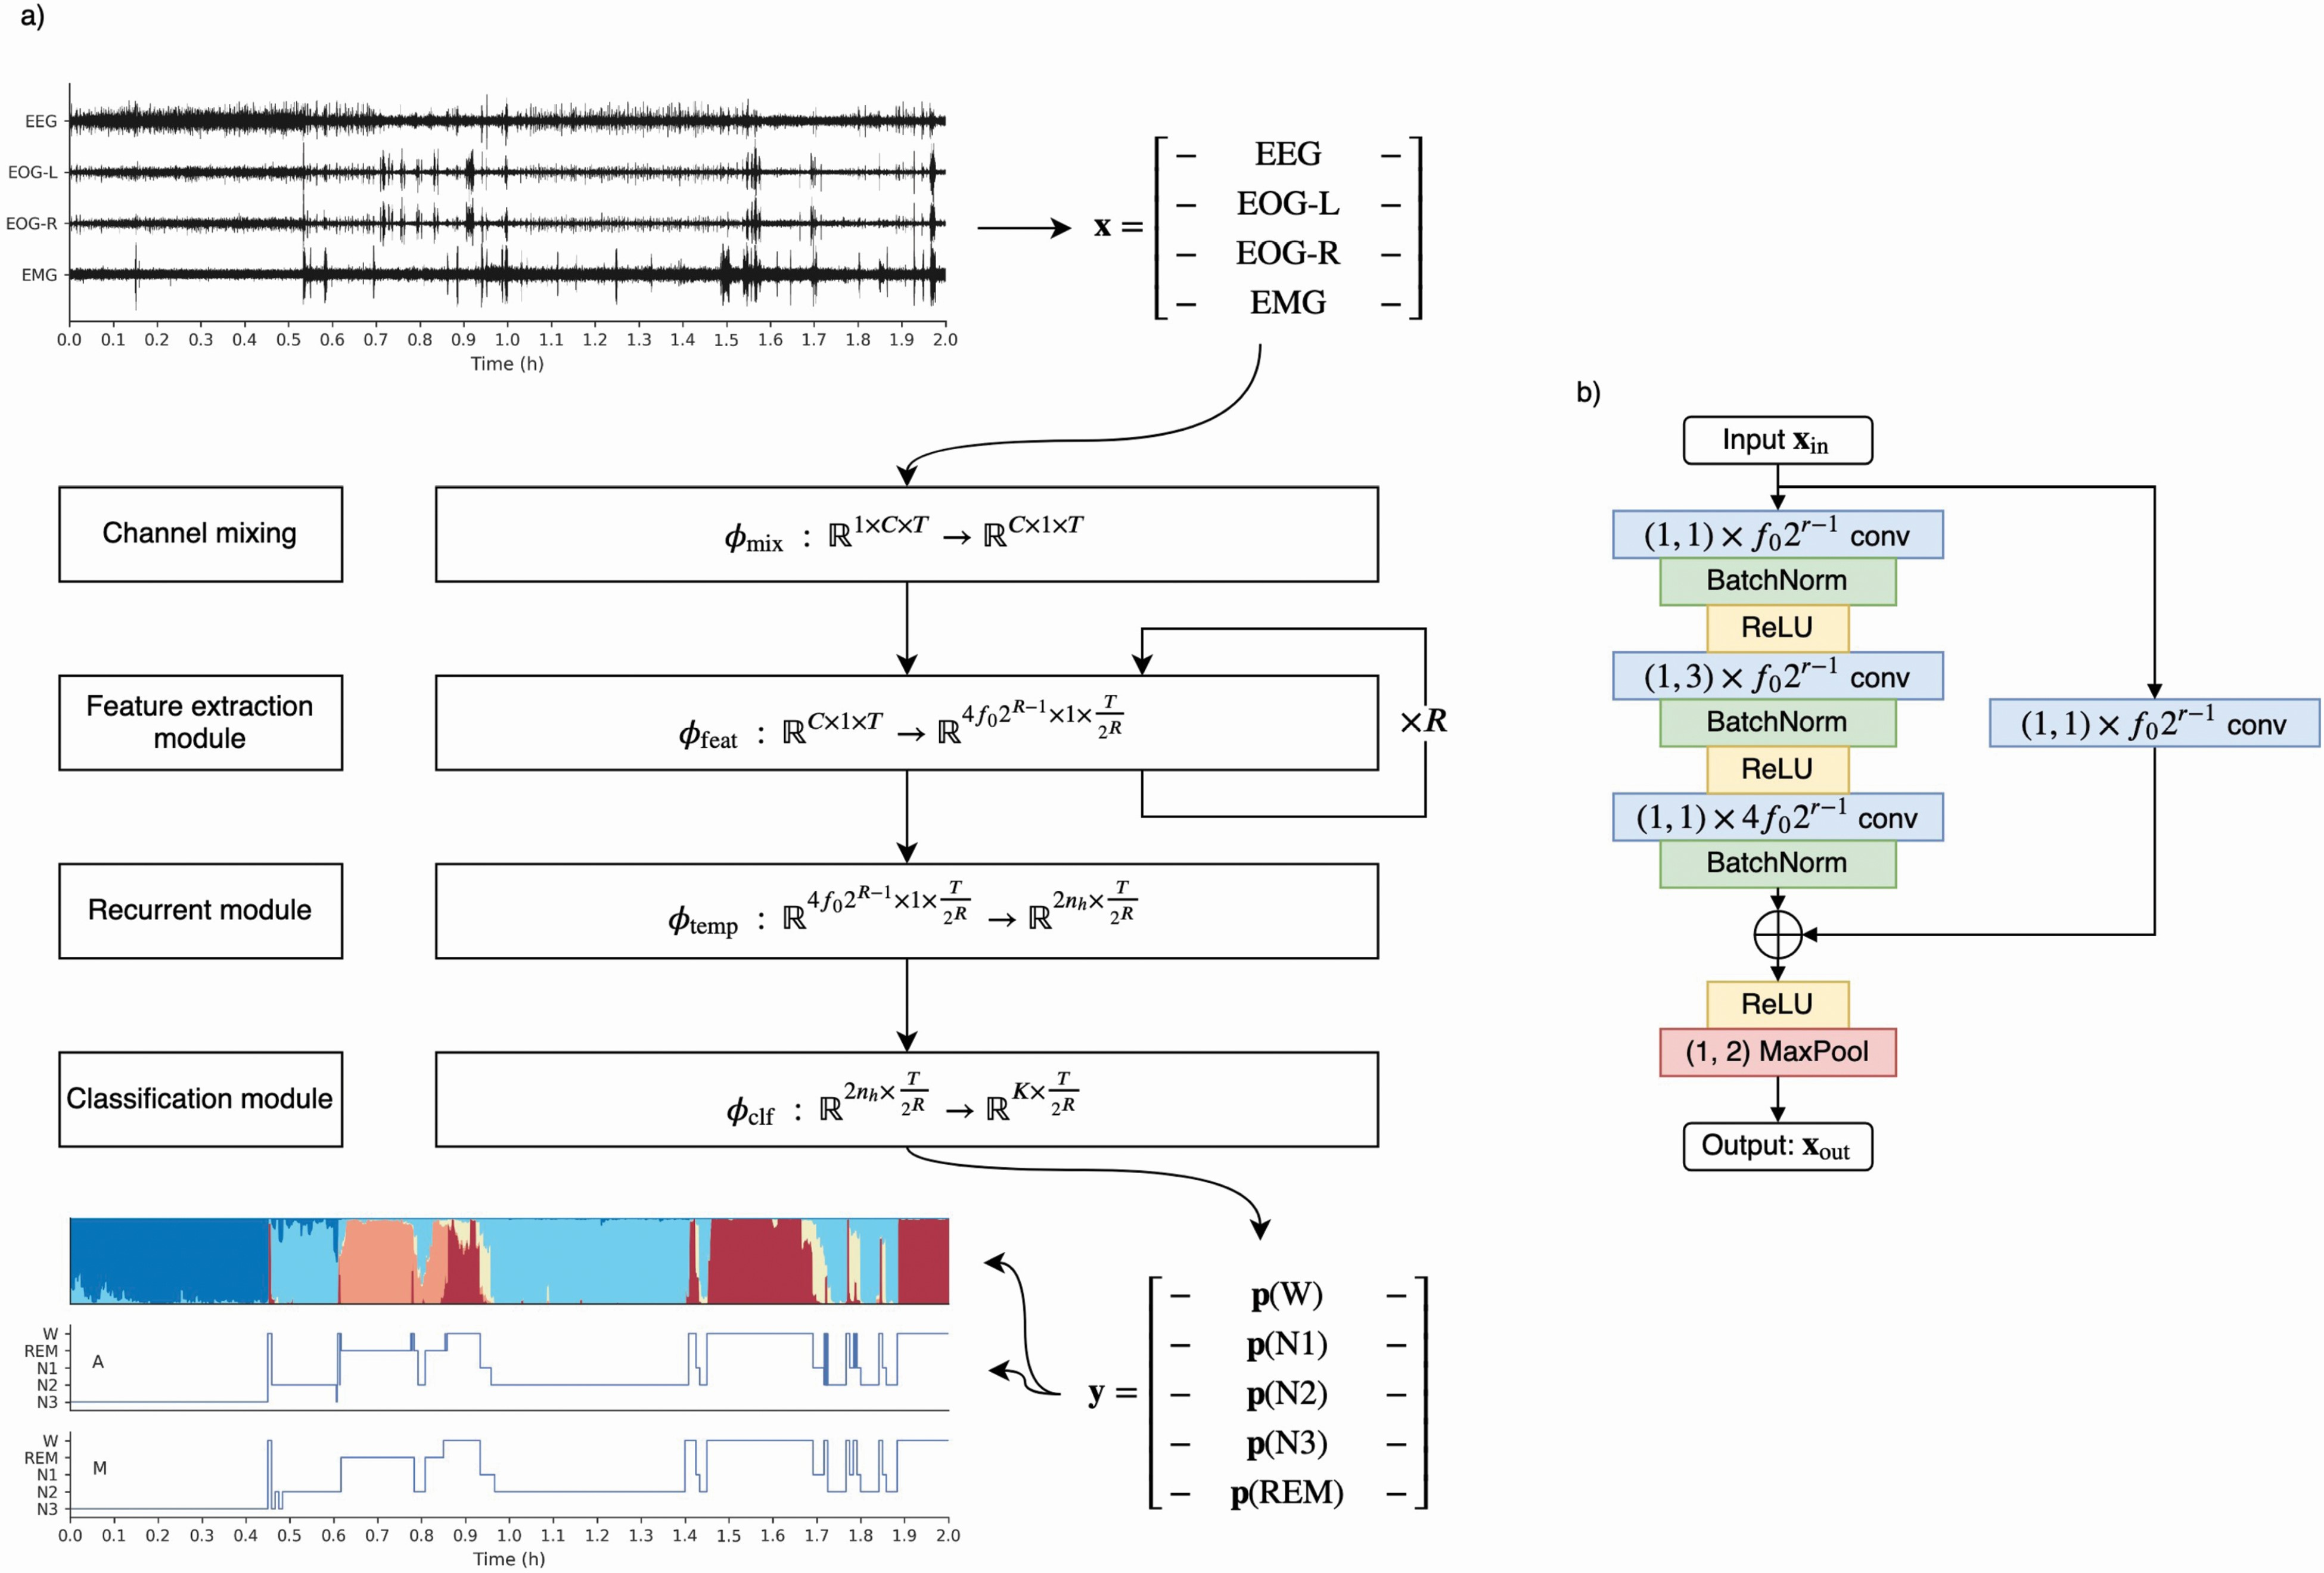
\includegraphics[width=0.8\linewidth]{Images/network_architecture.jpg}
    \caption{Network architecture used in \cite{Alexander2020}}
    \label{fig:network_architecture}
\end{figure}


\subsubsection{Steps of the pipeline}
A lot of the code used for this project, as well as the learned weights for the best model of the paper were made public though a GitHub repository \cite{Alexander2020}. Instructions on how and what to run in the pipeline are also available. Some essencial steps in the pipeline are:
\begin{itemize}
    \item \textbf{Setting up the PSG data .edf files} to be read in a folder and modify a config file to let the pipeline know the new location of the data. 
    \item \textbf{Latel identification}, by running a simple script that lets us map each electrode in our data to each electrode required by the pipeline, because there might not be a 1:1 correspondence between these.
    \item \textbf{Generate .h5 files from the data}, by running another script. Including modifying the code to extract the relevant patient metadata and data from our edf files. This step generates one h5 file for each subject, that includes the polysomnography data and ground truth hypnogram (if one was provided), as well as a .csv file for the cohort, with subject ID and file path information for each subject.
    \item \textbf{Inference on new data}, by calling the predict function with the learned weights on the h5 files, mentioning another config file. This generates .pkl files with the predicted sleep stage for each timestamp in the the PSG data, and performs some comparative metrics with the labeled hypnogram (if one was provided).
\end{itemize}



\subsection{Modifications to the pipeline} %===========================================================================
% Git hub and organization
The first step of coding for this project was to fork the original GitHub repository \cite{Alexander2020} to keep all of the original content while allowing to develop on top of that, keeping the coherence and structure The repository is available in \href{https://github.com/pplvieira/deep-sleep-pytorch-forked}{https://github.com/pplvieira/deep-sleep-pytorch-forked}. However some modifications had to be made on the code, and some envolved copying script files and hard coding some modifications on them, in order to fit some incompatibilities between the pipeline and our data and objectives for the project.
% LIBRARIES AND PYTHON VERSION
The scripts developed were run in the command line with Python 3.9.13, with notable libraries being matplotlib 3.7.1, yasa 0.6.5, scikit-learn 1.1.2 and pandas 2.1.0.

% Polysomnography
First, it is important to mention that the model was trained on polysomnography data. Meaning that it includes scalp EEG electrodes, as well as chin EMG and eletrooculogram (EOG). On the other hand, the data we have been acquiring is only from EEG channels.
Because of that, when mapping the channels from our data to the channels in the pipeline, the chin EMG and and EOG were left blanck, meaning that, after preprocessing of the channels, 1 out of the 4 data values that was passed to the model for each timestamp was zeroed out. 

% Lack of hypnogram
Another important incompatibility is that all throught the pipeline, it expects there to be a valid labeled hypnogram for the corresponding .edf file. However, the goal of this project was to perform predictions on new, unlabeled data, and comparing to the predictions from another pipeline to assess their agreement, not comparing with the ground truth (which was not available, as it would require a trained technician and a lot of time to annotate).
To work around this incompatibility with the pipeline, 2 of the python files were modified to \textbf{1:} produce a blank (all zeros) dummy hypnogram with the same size as the EEG data (instead of reading th hypnogram data from another .edf file) and \textbf{2:} ignore the comparison between predicted and "true" hypnogram at the end of the code, providing only the predictions, that would be compared to the results from other pipelines later.



\subsection{Additions to the pipeline} %===========================================================================
On top of the prediction pipeline, a few postprocessing and visualization scripts were made, to better visualize the results, manipulate the data and compare to other pipelines. These files, all located in a subfolder on the repository, are to be run as python scripts or modules, and include the \texttt{-h} flag and some other configurations to be called when running the code.

The scripts created are:
\vspace{-0.3cm}
\begin{itemize}
    \item \texttt{display\textunderscore hypnogram <predictionspath> --eval-window 30 --begining-index 0}: that simply manually retreives one predictions.pkl file (given in \texttt{predictionspath}) and plots the predicted hypnogram, as well as the distribution of the predicted relative probabilities of each sleep stage for each timestamp. The hypnogram is ploted using Yasa's \texttt{plot\_hypnogram} function \cite{2021yasa}.
    The eval-window can be change to perform averaging over the second-wise predictions in a smaller or larger window, the default, and most commonly used in the literature, is 30 (windows of 30 seconds). The time series of predictions is devided into chunks with size equal to the window size, and the predicted sleep stage for each chunk is the sleep stage with the highest probability inside all timestamps of that chunk of time. A larger window makes the output smoother but also loses time resolution. The begining index can also be changed, if, for example, the begining of the data corresponds to an awaken state, is too noisy or unpredictable and could be discraded for visualization.


    \item \texttt{predictions\textunderscore to\textunderscore txt --eval-window 30 --config <config>.yaml --prediction-dir \\ <predictdir> --output-dir <outputdir>}, which, for every file in the specified directory, converts the predictions.pkl into a .txt file in a lightweight and easy-to-read format, to be compared to other pipelines. This file format has one row for each epoch, with each row containing the predicted sleep stage. This step was included to make comparing results with other pipelines easier and streamlined, as the sleepEEGpy sleep staging wrapper \cite{belonosov2023sleepeegpy} exports the predicted hypnogram in this format. This function has a number of keyword arguments:
    \begin{itemize}
        \itemsep-0.4em
        \item \texttt{--eval-window}, that does the same as explained for the previous function (controling the size of each epoch), defaulted to 30.
        \item \texttt{--config}, references the .yaml file that was also used for obtaining the predictions in the original pipeline
        \item \texttt{--prediction-dir}, with the directory of all the .pkl predictions files, to be converted into the simple .txt format.
        \item \texttt{--output-dir}, with the directory of where the .txt files should be placed.
    \end{itemize}


    % dont know what im saying here
    \item \texttt{hypnogram\textunderscore comparison --folder <folderpath>}, which performs multi-rater analysis on multiple sleep staging predictions (from multiple different pipelines), each produced independently from the same .edf sleep EEG data. This function receives the folder of the .txt to be analyzed files as input. The .txt files presented can have different sizes (if for example 2 different window sizes were used for the same data), and the code will replicate the predictions of each file the number of times necessary for their duration to match (essencially make each file the size of the least common multiplier between their original sizes).
    %, but the sizes should be multiples of each other. 
    This script produces some plots:
    \begin{itemize}
        \itemsep-0.3em
        \item A confusion matrix for pairwise comparison of the predictions made by 2 of the raters for each timestep.
        \item A hypnogram comparison between which sleep stage each rater (each pipeline) has predicted for each time step, visualized as all hypnograms' time series superimposed as a function of time.
        \item A barplot with the proportion of number of agreers for each time stamp. Essencially telling, on how many timestamps do all the models agree.
        \item A matrix of inter-rater agreement (accuracy), essencially saying how much each pair of raters agree with each other (in case there are more than 2 raters).
        \item A matrix of inter-rater Cohen's kappa score, essencially the same as the previous, but with the Cohen's kappa instead of agreement.
    \end{itemize}
\end{itemize}

% mathematical defnitions of agreement and kappa
Using the notation from section \ref{section:mathematical_definitions}, given $M$ different raters (or different prediction pipelines) and $N$ epoch predictions from each, we want to define some metrics to compare the predictions between all of them. 
With $\mathbf{S^{\prime}}_{(l)}$ being the predicted hypnogram from rater $l$, we define $C^{(lm)}$ as the joint hypnogram between raters $l$ and $m$. I.e. $c_{ij}^{(lm)}$ is the number of epochs where rater $l$ predicts label $i$ and rater $m$ jointly predicts label $j$.

We then define agreement ($\text{Acc}^{(lm)}$) as the proportion of pairwise predictions that match between a pair of raters $l$ and $m$ (eq.\ref{eq:accuracy_definition}). 
\begin{equation}
    \text{Acc}^{(lm)} = \frac{\sum_{i} c_{ii}^{(lm)}}{\sum_{i,j} c_{ij}^{(lm)}}
    \label{eq:accuracy_definition}
\end{equation}
\vspace{-0.2cm}


Simillarly we define Cohen's kappa score between a pair of raters $l$ and $m$ ($\kappa^{(lm)}$), which takes into consideration the chance of the raters agreeing, and is a more robust measure of inter-rater reliability than accuracy. A kappa score of $\geq0.8$ is already considered almost perfect agreement. For $k$ categories, $N$ epochs to categorize and $n_{ki}$ the number of epochs where rater $i$ predicted category $k$:
\begin{equation}
    \kappa^{(lm)} = \frac{\text{Acc}^{(lm)} - p_e^{(lm)}}{1 - p_e^{(lm)}} \ , \quad p_e^{(lm)} = \frac{1}{N^2} \sum_{k} n_{kl} n_{km}
    \label{eq:kappa_definition}
\end{equation}
\vspace{-0.3cm}






\subsection{Pipeline features} % ??? %===========================================================================
\begin{figure}[H]
    \centering
    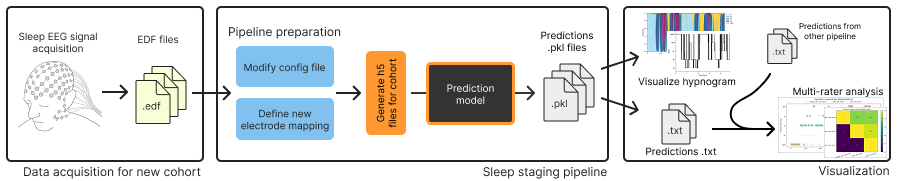
\includegraphics[width=1\linewidth]{Images/pipeline_diagram2.png}
    \caption{Simplified diagram of the full pipeline}
    \label{fig:pipeline_diagram}
\end{figure}
\vspace{-0.5cm}

% sequence + flexibility / tried to make it as readable as possible for the posterity
With this, we arrive at the final pipeline developed for this project, essencially consisting in a wrapper around the sleep staging pipeline in \cite{Alexander2020}. Fig.\ref{fig:pipeline_diagram} includes a schematic of the full pipeline. The 3 big blocks are essencially independent and almost isolated, and should be applied in sequence. Ensuring readability and ease of use for the posterity was also taken in consideration, in case automatic sleep staging continues to be of interest to Optoceutics and as more data is acquired through the years. 

% in more detail
The sleep data can be recorded through time with the protocol being used by Optoceutics and the research, and introduced into the pipeline as more and more data is gathered. The pipeline preparation steps only need to be done once for a new cohort of data, with cohort meaning a set of EEG .edf files with the same electrode setup and recording settings. As more data is introduced, generating the cohort files and passing them through the sleep staging prediction model is done by running 2 commands in the local terminal. The visualization part of the pipeline allows for manual visualization of the prediction results as well as small processing and comparison with the predictions from other pipelines, for a multi-rater assessment.

% what we can change (psg, swap model, compare to any prediction)
The parameters used on the pipeline preparation block for this project assumed the data consisted of a simple EEG recording, not a full polysomnography, to ensure consistency with the recordings we were provided. However, this results in loss of information, and most certainly in worse prediction results as well. If Optoceutics eventually acquires full polysomnography data, running the electrode mapping function again would ensure the information is not lost.
Aditionally, the prediction model is represented by a black box in the pipeline, as we are agnostic to the functioning of the model. It could also be swapped by another model as long as they take the same format of input and output. 
Finally, the multi-rater comparison can essencially be done with any number of other pipelines, as long they can be converted into the afformentioned .txt format. The analysis can also be done with manually labeled hypnograms if they are eventually obtained for Optoceutics' sleep recordings, meaning the prediction model or the data gathering could be validated. 

% COOPERATION + GOAL~~~
Finally, this project was done with a lot of colaboration from a collegue, who assessed the quality of another automatic sleep staging pipeline, using sleepEEGpy \cite{belonosov2023sleepeegpy}, a wrap around of another sleep staging Python library: YASA \cite{2021yasa}. The multi-rater analysis part of the pipeline developed here was mostly used to compare the results from each of the 2 pipelines, and because labeled sleep EEG data was unavailable, agreement between the raters was considered as a good enough proxi for the ground truth. In fact, as one the goal of the project was to expand Optoceutics' library of labeled sleep EEG data, and to assess the feasibility of further sleep studies, this multi-rater setup was more than enough.








%\newpage
\section{Results and discussion}

% results from my pipelines automatic sleep staging
% no ground truth but multirater cooperation. hypnogram comparison with patricia, metrics, conf matrices
% hypnogram comparison with GT for sleepEDFdatabse



% only 2 recordings
In total, only 2 overnight EEG sleep recordings (from 2 different healthy adult makes) were used in the pipeline during the course of this project. They were produced in the European Data Format (.edf). The recordings were taken from a 27 channel EEG setup used interally for clinical trials. 
However, as was described, the pipeline is prepared to receive more data, and obtaining the predictions for them is streamlined.
\\
% redundant to report on all
Reporting on all sleep recordings is, therefore, slightly redundant, as the goal was not to obtain good results for one patient, but streamlining obtaining those results for a cohort of subjects fast and efficiently. With this, only the results for one of the subjects will be shown on most plots, to be used as an ilustrative example of the pipeline's functioning and output formats. 


\subsection{Sleep staging results}
% hypnogram results
From the \texttt{visualize\_hypnogram} script, the hypnogram  (Fig.\ref{fig:hypnograms_30_120}) and prediction probabilities plot (Fig.\ref{fig:hypnogram_probs_30}) are produced based on the predictions.pkl files for each subject, which are the output of the pipeline in \cite{Alexander2020}.

\vspace{-0.2cm}

% hypnograms with 2 windowsizes
\begin{figure}[H]
    \centering
    \begin{subfigure}[b]{0.46\textwidth}
        \centering
        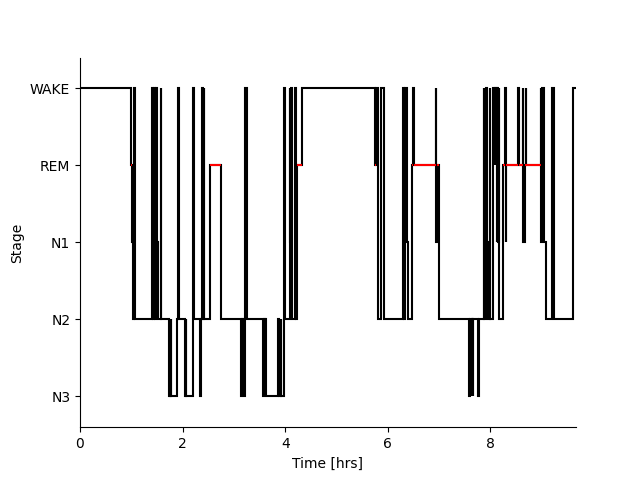
\includegraphics[width=\textwidth]{Images/marcus_hypnogram_30.png}
        \caption{Hypnogram with window of 30 epochs}
        \label{fig:hypnogram_30}
    \end{subfigure}
    \hfill
    \begin{subfigure}[b]{0.46\textwidth}
        \centering
        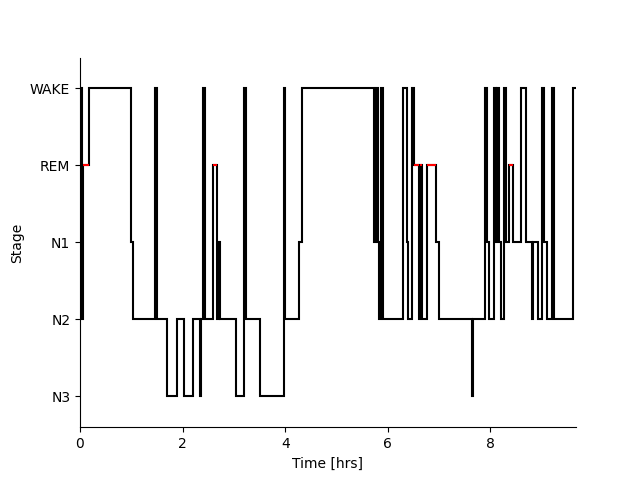
\includegraphics[width=\textwidth]{Images/marcus_hypnogram_120.png}
        \caption{Hypnogram with window of 120 epochs}
        \label{fig:hypnogram_120}
    \end{subfigure}
    \vspace{-0.1cm}
    \caption{Predicted hypnograms for the same data, for 2 window sizes}
    \label{fig:hypnograms_30_120}
\end{figure}


% probs hypnogram
\vspace{-1cm}
\begin{figure}[H]
    \centering
    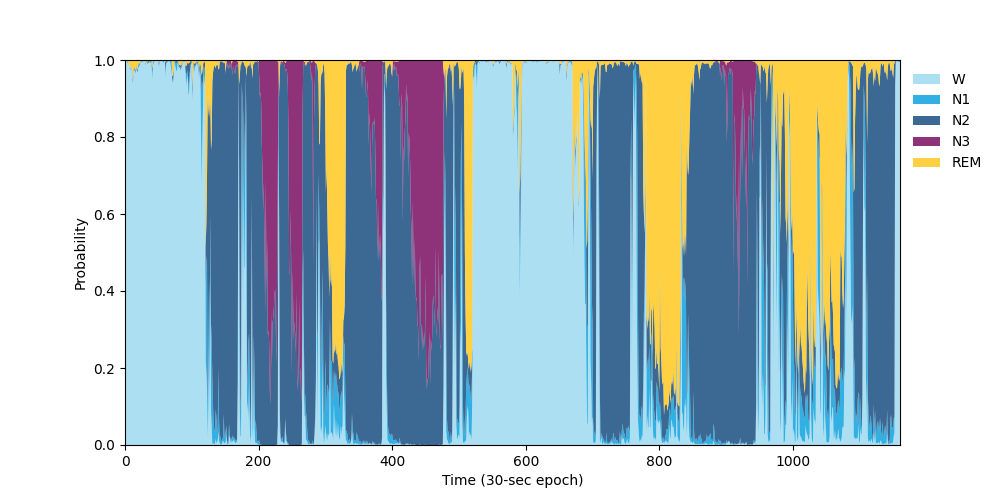
\includegraphics[width=0.7\linewidth]{Images/marcus_hypnogram_probs_30.png}
    \caption{Probabilities for each sleep stage for each epoch}
    \label{fig:hypnogram_probs_30}
\end{figure}

% explain the 2 windowsizes
The results from Fig.\ref{fig:hypnogram_30} and Fig.\ref{fig:hypnogram_120} were obtained by running the \texttt{display\_hypnogram} twice, with different window sizes. A initial index of 18000 was also used, as the recording had a few hours where the subject was still awake. As expected, the result with a bigger window (2 minutes) is smoother but loses a lot of time resolution. Namely, the amount of predicted REM sleep is almost halved with a bigger window. This stage of the sleep cycle can sometimes be very short ($\sim$5 minutes), and the bigger window might have a harder time picking it up.

% explain the probas plot
On the other hand, Fig.\ref{fig:hypnogram_probs_30} shows the predictions' confidence of each sleep stage for each 30 seconds epoch. In essence, each point in the hypnogram in Fig.\ref{fig:hypnogram_30} is the sleep stage with the highest probability for that epoch from the predicted hypnogram probabilities (Fig.\ref{fig:hypnogram_probs_30}).





\subsection{Multi-rater comparison}
% explian where the data came from
For the multi-rater comparison of results from different pipelines, it was imperative that the predictons from each were in the same format. Because the results from the pipeline used by my collegue (\cite{2021yasa,belonosov2023sleepeegpy}) automatically exported the predictions in the txt format mentioned (with the prediction for each epoch in each line), running the \texttt{predictions\_to\_txt} on the predictions from this pipeline would ensure coherence. Like for visualizing the hypnogram, the \texttt{predictions\_to\_txt} script was run twice with 2 different values for the evaluation window: 30 and 60 seconds. After placing these 2 txt files (\texttt{subj-1\_win-30.txt} and \texttt{subj-1\_win-60.txt}) as well as the one produced from the other pipeline (\texttt{model2\_subj-1\_win-30.txt}), all 3 obtained from the same sleep EEG data, in the same folder, running the \texttt{hypnogram\_comparison} script produced the plots below. It is important to mention that, as the first two files were produced from the same predictions but with different sizes of prediction windows, the results between these two were expected to be quite simillar, and were included side to side as a form of control.



% TALK ABOUT THE SUPERIMPOSED AND CM
In Fig.\ref{fig:multirater_hypnogram}, the superimposed predicted hypnogram for each of the 3 models is shown. Together with the confusion matrix of preditions between \texttt{model2\_subj-1\_win-30} and \texttt{subj-1\_win-30}, we show that these two models agree on most pairs of predictions, most notably in the wake and REM stages. Cruacially, there seems to be less agreement in the light and deep sleep, with model 1 \cite{Alexander2020} predicting more light sleep (N1) and model 2 \cite{2021yasa} predicting more deep sleep, in general.

% number of raters
Due to the lack of real annotated data, the number of raters that agree on the predicted sleep stage for a certain time stamp is a good proxi for the confidence on the prediction of the ensemble. And, if all raters, i.e. all automatic sleep staging algorithms used, agree on a certain prediction, we could, to a certain degree of confidence, assume that as the true predicted label for that time stamp. Fig.\ref{fig:number_of_agreers} shows that on 85\% of the time, all 3 predictions agree, which is already a good sign that the predictions are not far from the truth.


% multirater hypnogram
\begin{figure}[H]
    \centering
    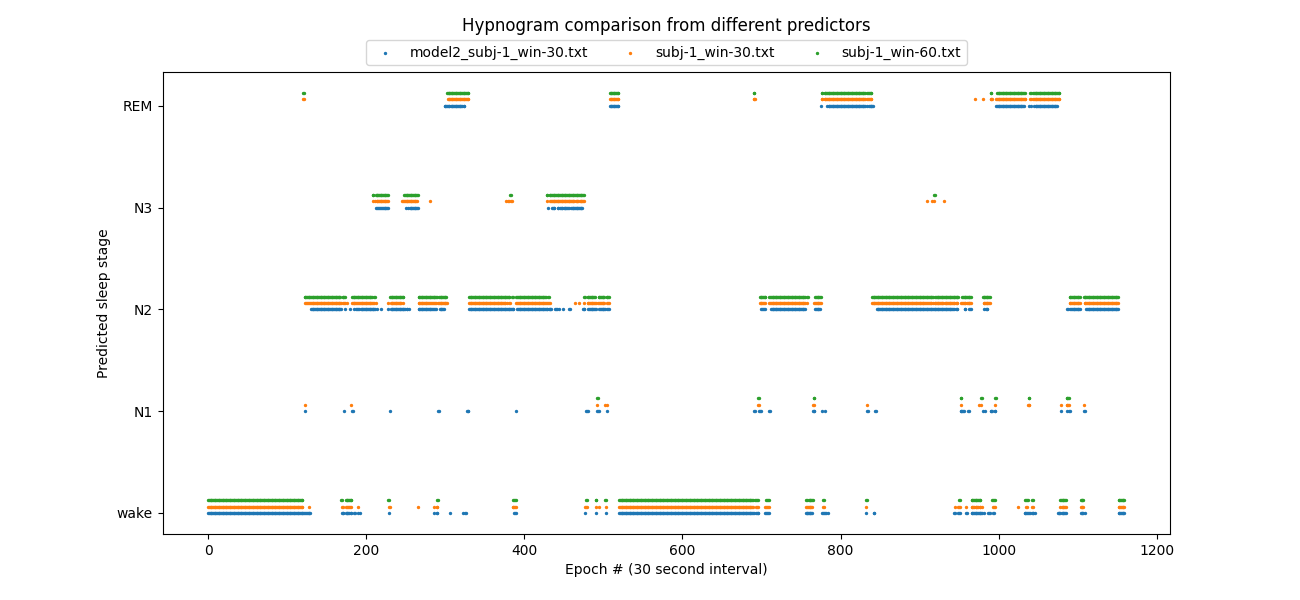
\includegraphics[width=0.99\linewidth]{Images/comparisson1_hypnogramComparison.png}
    \vspace{-0.8em}
    \caption{Multi-rater hypnogram predictions}
    \label{fig:multirater_hypnogram}
\end{figure}



% CM for all predictions between 2 models
\vspace{-0.9cm}
\begin{figure}[H]
    \centering
    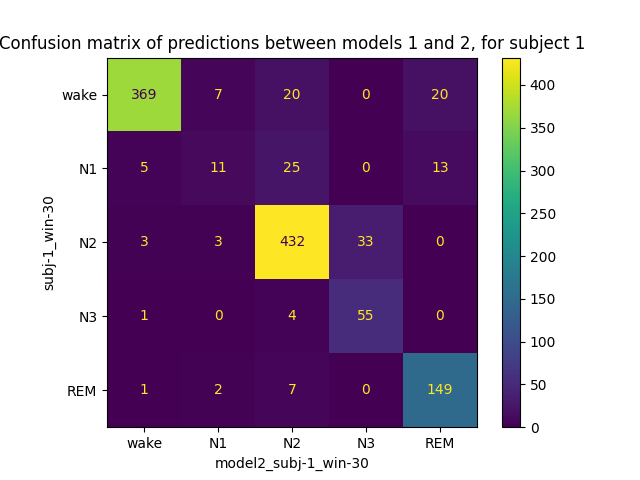
\includegraphics[width=0.55\linewidth]{Images/comparisson1_predictionsCM.png}
    \vspace{-0.8em}
    %\caption{Probability of 1, 2 or 3 of the predictions agreeing for any time stamp}
    \caption{Confusion matrix for all epoch predictions between \texttt{model2\_subj-1\_win-30} and \texttt{subj-1\_win-30} }
    \label{fig:CM_between_2_raters}
\end{figure}



% number of agreers 
\vspace{-1cm}
\begin{figure}[H]
    \centering
    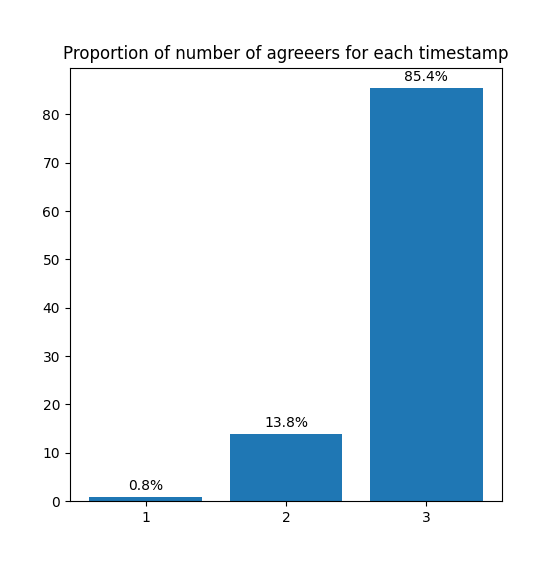
\includegraphics[width=0.4\linewidth]{Images/comparisson1_numAgreers.png}
    \vspace{-1em}
    %\caption{Probability of 1, 2 or 3 of the predictions agreeing for any time stamp}
    \caption{Percentage of time stamps where none, 2 or all 3 prediction models agree}
    \label{fig:number_of_agreers}
\end{figure}



% agreements and kappa score
\begin{figure}[H]
    \centering
    \begin{subfigure}[b]{0.48\textwidth}
        \centering
        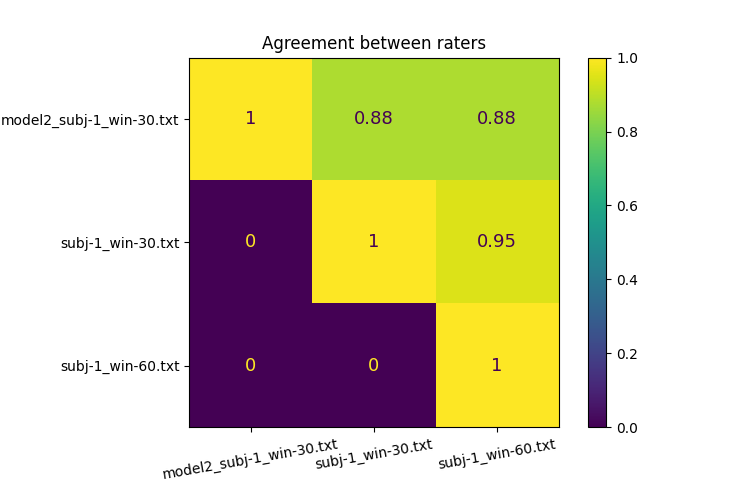
\includegraphics[width=\textwidth]{Images/comparisson1_accuracyCM.png}
        \caption{Agreement between each pair of raters}
        \label{fig:multirater_agreementCM}
    \end{subfigure}
    %\hfill
    \hspace{-0.5cm}
    \begin{subfigure}[b]{0.48\textwidth}
        \centering
        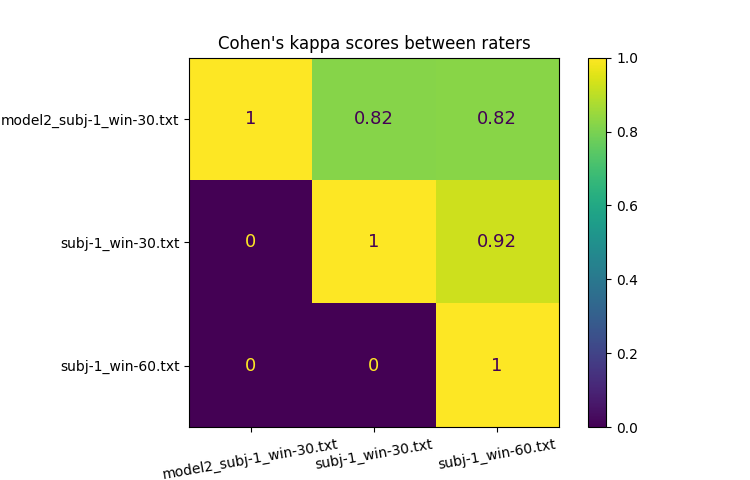
\includegraphics[width=\textwidth]{Images/comparisson1_kappaCM.png}
        \caption{Kappa score between each pair of raters}
        \label{fig:multirater_kappaCM}
    \end{subfigure}
    \caption{Agreement and Kappa scores between each pair of raters}
    \label{fig:multirater_CMs}
\end{figure}


% CM of agreement and of kappa - EXPLANATION
Fig.\ref{fig:multirater_agreementCM} shows the percentage of agreement between each pair of models. Likewise, Fig.\ref{fig:multirater_kappaCM}, shows the Kappa score between each pair of model predictions. 
The diagonal of the matrix is, by definition, just ones, and the lower triangular matrix was displayed as zeros to avoid confusion, but the matrices are essencially simetrical because both agreement and Kappa score are invariant to changing the order of the pair of models.

% CM of agreement and of kappa - IN DEPTH
As expected, the agreement and Kappa score are almost 1 between \texttt{subj-1\_win-30} and \texttt{subj-1\_win-60} (0.95 and 0.92 for agreement and kappa, respectively). 
Both metrics were the same between any of the predictions with different window sizes from model 1 and the predictions from model 2 (0.88 agreement and 0.82 kappa score). 
With all this, the multi-rater ensemble-like setup demonstrated quite good levels of agreement between multiple models, and proved to be a satisfactory automatic sleep staging algorithm.



% RESULTS FOR OTHER PATIENT TESTED
\subsection*{Results for subject 2} %\#
The results from performing the same analysis on the second subject were not displayed, but some analysis can still be done. The agreement and kappa score between the pipeline used here and the pipeline used by my collegue were of 0.77 and 0.64, which is slightly lower than for the first subject. The 2 raters had quite good agreement with N2 and awake states, but performed poorly on the other sleep stages. Fig.\ref{fig:Appendix_subj2_multirater_hypnogram} in the appendix shows the hypnogram each of the 2 models predicted, superimposed.




\subsection{Validation with ground truth dataset}
% why do this
Finally, a small validation study on a simple EEG sleep dataset with annotated hypnograms was done. This exercise was do to try to validate the model and pipeline in a labeled dataset consisting in sleep data more similar to the EEG setup being used in Optoceutics' research. In other words, to assess if this model performed well enough against EEG only annotated data.

% only one datapoint and how to run
For this analysis, due to lack of time, only the first entry in the sleep EDF database \cite{kemp2018sleepEDFwebsite,2000sleepEDForiginal} was used. The steps of the pipeline were run in sequence as prescribed, treating the new data as a new cohort. In the end, instead of comparing the predicted hypnogram from 2 different raters, the results from this pipeline were compared to the labeled hypnogram. 

% results
The small validation study provided satisfactory results, with accuracy of 78\% but a Cohen's kappa score of only 0.55. The side by side hypnogram comparison as well as the confusion matrix between the predicted and ground truth labeled data can be found in the appendix (Fig.\ref{fig:Appendix_GT_hypnogram} and Fig.\ref{fig:Appendix_GT_CM}). The prediction model tended to overpredict the REM stage when the patient should have stil been awake, but the N2 and especially N3 were predicted relatively accurately. Another relevant finding is that, while the prediction model oscilates between different predictions in sequential 30s epochs, the ground truth is far more smooth and continuous.



%\newpage
\section{Conclusion}



%\subsection{????}


\subsection{Shortcomings of this approach} % no GT
% bootstrap
Even though the results were promising and the pipeline performs as intended, the implementation was strongly bootstrapped given all the limitations and incompatibilities between all the moving parts. Some incompatibilities were ignored or overwritten, and there were no real validated results and very little data.

% didnt have PSG data
Arguably the most important limitation with this implementation is that the automatic sleep staging algorithm in \cite{Alexander2020} was trained on PSG data, namely central EEG, left and right EOG, and a single submentalis EMG. The prediction algorithm expected 2 time-series channels of EEG data, one of EOG and another of chin EMG. However, the data we had access to only had scalp EEG recordings, meaning that a suspected 1/4 of the data (corresponding to the chin EMG) used for the predictions was blanck, most certainly leading to inaccurate results. 

% still had good results though
Nonetheless, the predictions had good agreement with the predictions from the Yasa model, which was trained only on EEG data, as well as good validated results on the sleepEDFdatabase simple EEG data.

% not that much data or need to validate at least some
Another consideration is that only 2 sleep recording were used during the course of this project. To test the feasibility and replicability of this pipeline, more data is needed, to produce mass data sleep stage predictions on Optoceutics' data.

% all boils down to lack of validation
In summary, there is a just a lack of validation in this pipeline. Even though each of the components (a standardized overnight EEG setup, a automatic sleep staging pipeline, and a data manipulation and visualization wrapper) are all validated or work as intended by themselves, there is no certainty that the EEG data gathered is adequate enough for the prediction model. There is no ground truth to compare out predictions in this setting to, and very little sleep data to make a statistical inter-rater comparison.

% lack of clinical usage
Finally, as has been reported in the literature, even tough automatic sleep staging with computational tools provides a massive improvement in throughput and labeling time, with accuracies close to those of manual annotators, it still hasn't been widely used in clinical applications \cite{2022automaticEEG}, which might be another barrier of this technology.  


\subsection{Future prospects}
% apply on more data + validate on more data
The first future prospect would be to apply the pipeline on a ever-increasing internal database of sleep EEG recordings. A lot of consideration was taken into making it as streamlined as possible to add more sleep EDF files and extract predictions and perform data analysis on those.
If given more time, it would also make sense to validate this pipeline on more than just one sleep recording from the sleepEDFdatabase, or other EEG based annotated sleep staging dataset, to get a better idea of the generalization capability of this model.

% try another model
The prediction model used was also the best model made available in \cite{Alexander2020}, with no finetuning. However, the pipeline is built to accept any pretrained prediction model as long as the input and output have the same shape as the one used here. Therefore, it would eventually be beneficial to either swap the prediction model for another one developed in the literature; finetune the model in \cite{Alexander2020} to our data; or develop and train a new model from scratch on validated data with the same EEG setup as the one used internally.


% eventually get it validated on our data
It would eventually be beneficial to have our automatic sleep staging validated by a professional. I.e. having a trained technician manually annotate one of the sleep EEGs used here and statistically comparing it with the automatic predictions. 



\subsection{Objectives acheived}
% theoretical objectives
The theoretical objectives of this project were certainly acheived, with additional insight gained into the mechanisms of Alzheimer's disease, neurostimulation and the glymphatic system. But most importantly, into sleep studies, automatic sleep staging in the literature and the importance of sleep in Alzheimer's disease pathophysiology.

% pipeline developed
The pipeline wrapper developed provides easy to use sequencial instructions and commands, to apply automatic sleep staging, visualize results and perform multirater comparison. The multi-rater analysis as well as the basic validation with the sleepEDFdatabase provided good levels of agreement, giving us some light into the accuracy of the whole setup.

% multirater setup is good
With all this, and given the lack of a true label on the sleep EEG data acquired, the multi-rater ensemble-like setup is not only satisfactory as a quick and effective automatic classification setup, but also demonstrated quite good levels of agreement between multiple models.



% ======================================================================================
\section*{Code availability}
\addcontentsline{toc}{section}{Code availability}
All the code developed, the wrapper pipeline and instructions can be found in the GitHub repository \\
\href{https://github.com/pplvieira/deep-sleep-pytorch-forked}{https://github.com/pplvieira/deep-sleep-pytorch-forked}

% ======================================================================================
\section*{Disclaimer}
\addcontentsline{toc}{section}{Disclaimer}
% \addcontentsline{toc}{section}{\protect\numberline{}Acknowledgments}
% \addcontentsline{toc}{section}{References}

A small disclaimer regarding copyright and plagiarism: this project was done with close colaboration with a collegue, Patricia Almeida also from DTU, and our reports will have some overlap in the dataset and overall approach. We each worked independently by applying 2 different automatic sleep staging pipelines on the same data, and part of the results and discussion will overlap on the multi-rater part of our report, as the predictions from both pipelines were merged to produce some of the results. This should not be considered plagiarism.

%I would like to thank everyone in Optoceutics for the opportunity to do this practical project course with them,


\newpage
\addcontentsline{toc}{section}{References}
%\bibliography{document.bib}  %%%% ESTA LINHA E A SEGUINTE ESTAVAM UNCOMMENTED!!!!


%\bibliographystyle{ieeetr}
\printbibliography




\clearpage


\appendix
\renewcommand\thefigure{\thesection.\arabic{figure}} 
\setcounter{figure}{0} 
\section{Appendix - Suplementary figures}
%\section{Appendix A - Suplementary figures}


% multirater hypnogram
\begin{figure}[H]
    \centering
    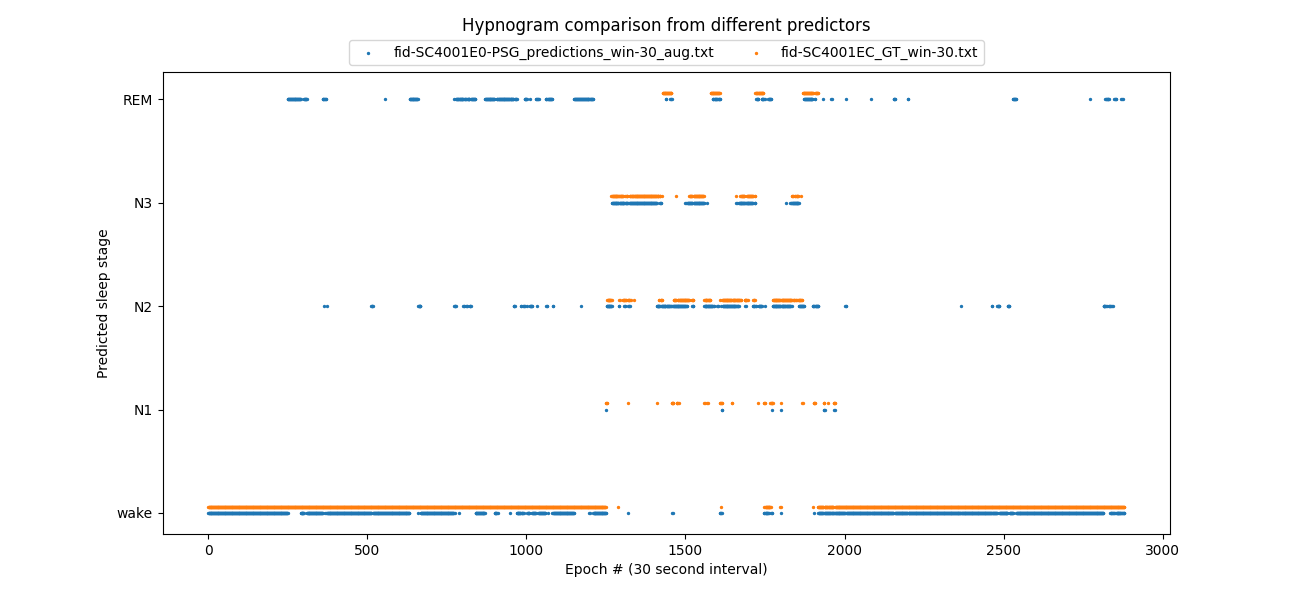
\includegraphics[width=0.99\linewidth]{Images/comparisonGT_hypnogramComparison.png}
    \vspace{-0.8em}
    \caption{Predicted (\texttt{...-PSG\_predictions\_...}, in blue) and ground truth (\texttt{...\_GT\_...}, in orange) hypnogram for sleep EDF database patient \#001}
    \label{fig:Appendix_GT_hypnogram}
\end{figure}



% CM for all predictions between 2 models
\begin{figure}[H]
    \centering
    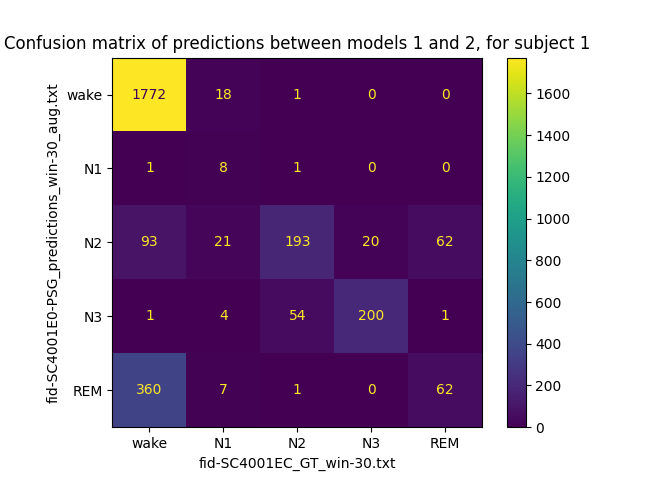
\includegraphics[width=0.6\linewidth]{Images/comparisonGT_predictionsCM.png}
    \vspace{-0.8em}
    %\caption{Probability of 1, 2 or 3 of the predictions agreeing for any time stamp}
    \caption{Confusion matrix for all epoch predictions between the predicted (\texttt{...-PSG\_predictions\_...}, across) and ground truth (\texttt{...\_GT\_...}, down) for sleep EDF database patient \#001}
    \label{fig:Appendix_GT_CM}
\end{figure}



% multirater hypnogram 2 subject
\begin{figure}[H]
    \centering
    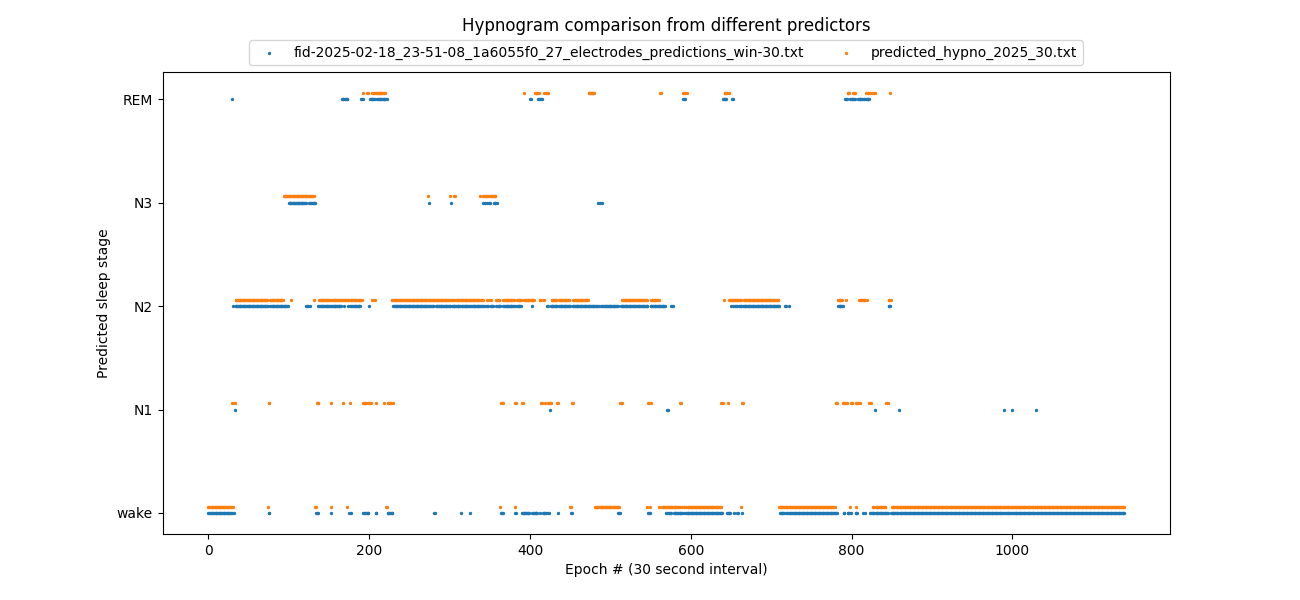
\includegraphics[width=0.99\linewidth]{Images/comparisson2_hypnogramComparison.png}
    \vspace{-0.8em}
    \caption{Multirater hypnogram comparison, with this pipeline's predictions (\texttt{fid\ ...\_predictions\_win-30...}, in blue) and Yasa's prediction (\texttt{predicted\_hypno\_2025}, in orange) hypnogram for subject \#2}
    \label{fig:Appendix_subj2_multirater_hypnogram}
\end{figure}




% \appendix
% \section{Appendix A - CNN definition, training and evaluation script}
% \lstinputlisting[style=Python,
%     caption=CNN definition, training and evaluation script,
%     label={RunTrain.py},
%     breaklines=true,
%   ]{RunTrain_.py}



% %\appendix
% \newpage
% \section{Appendix B - model reader and weight visualization script}
% \lstinputlisting[style=Python,
%     caption=model reader and weight visualization script,
%     label={VisualizeWeights.py},
%     breaklines=true,
%   ]{VisualizeWeights.py}

%\bibliographystyle{aomplain}
%\bibliographystyle{vancouver}
\label{EndOfText}


%\newpage
%\pagenumbering{Roman}
%\fancyfoot[C]{Page \thepage\ of \pageref{EndOfAppendix}}
%\input{sections/0_code}
%\label{EndOfAppendix}

\label{endOfDoc}

\end{document}
